%=======================================================================================%
% the main points of this introduction are 
% outline the complexity of biological systems for physicists
% 	> even though our theoretical models should preidct everything on the energy and length scales of biology we can't because of their heterogeneity.
%   > Give examples of the heterogenaity 
% Give some points on the history of molecular biophysics  
%   >  Hodgkin-Huxley Models
%   > Gramicidin 
% Point out how Cystic Fibrosis is an expression of this progression, going from genotype to phenotype using an ion channel to teach us biophysics. 
% conclusion.
\chapter*{Foreword}
\markboth{Foreword}{Foreword} 
%\lhead{\emph{Foreword}}
\label{chap:foreword}
\begin{chapquote} {}
I've never held a pipette
\end{chapquote}

The more I wrote of this thesis the more I found myself writing down things I wish I had known when I first started studying biophysics. I was writing for my past self. So I've tried my best to write each chapter to be understandable to those with a loose grasp of undergraduate physics. The most difficult thing for this audience will not be the mathematics or technical content herein, but rather the breadth of knowledge from different fields to understand the scope of the contents. I have not had time to write an introduction to molecular biology, so I recommend a physics based introduction to those concepts such as those found in ``The Physical Biology of the Cell" \cite{phillips2012}. For more intensive biology focussed introduction there is ``Cell Biology"\cite{pollard2016}. In this spirit of trying to give the reader an interdisciplinary roadmap, I have taken some care to name certain authors as waypoints, to give the reader anchors to help them navigate the literature. Similarly, when a technical concept is mentioned, I have searched for a useful review article, book or explainer. So please take such citations as reading recommendations \cite{dawkins1989, hofstadter1999}.

\begin{figure}[h]
	\begin{center}
		\includegraphics[width=0.9\textwidth]{figures/myelin.jpg}
	\end{center}
	\captionsetup{singlelinecheck = false, justification=raggedright}
	\caption[Nerve Cross Section by David Goodsell] {\textbf{Nerve Cross Section by David Goodsell}}{David Goodsell is an artist who produces water paintings of cellular environments. Many of his works can be downloaded and used \href{https://pdb101.rcsb.org/sci-art/goodsell-gallery}{for free}. He has also written many books and articles which would serve as a light, layperson friendly introduction to molecular biology \cite{goodsell2009, goodsell2018, goodsell2020}. This particular painting depicts the cross section of a nerve. The nerve fibre (blue) is wrapped in an insulating myelin sheath (yellow). Electrical signals propagate perpendicular to the page, via voltage gated sodium and potassium protein ion channels at the edge of the nerve\cite{goodsell_nerve}. We will discuss the discovery and details of this mechanism in the next chapter, as they were critical to the development of biophysics.}
	\label{goodsell_figure}
\end{figure}

When I first started performing simulations of living systems, I didn't even know what a protein was, and as I'm writing this, I have still never taken a formal course in biology or chemistry. Despite this, for the past 4 years I have been captivated by the seemingly infinite complexity in biological systems. For some examples, please take this opportunity to treat yourself to the fabulous work of \href {https://pdb101.rcsb.org/sci-art/goodsell-gallery}{David Goodsell} in Figure \ref{goodsell_figure}.\footnote{\href{https://pdb101.rcsb.org/sci-art/goodsell-gallery}{https://pdb101.rcsb.org/sci-art/goodsell-gallery}} 

Overall, I've found that the mindset for solving biological problems feels very different to the narrowed focus which we cultivate in students to study idealised problems in mathematics and physics. The problems are more specific and the solutions are often less general. For example, plasma physicists may use the same mathematical tools to describe a diverse set of materials, from the dense stellar core, to the sparse intergalactic nebulae. The density of these objects spans 28 orders of magnitude \cite{chen2018}.\footnote{From $10^{34}-10^6$ charged particles per meter cubed respectively.} Would that we were so lucky in biology, where we struggle to apply same physical models to deal with phenomenon across a single order of magnitude. All the same, it seems increasingly clear to me that living things as we understand them occupy a special place in the universe (Figure \ref{length_scales}). 


\begin{figure}
	\begin{center}
		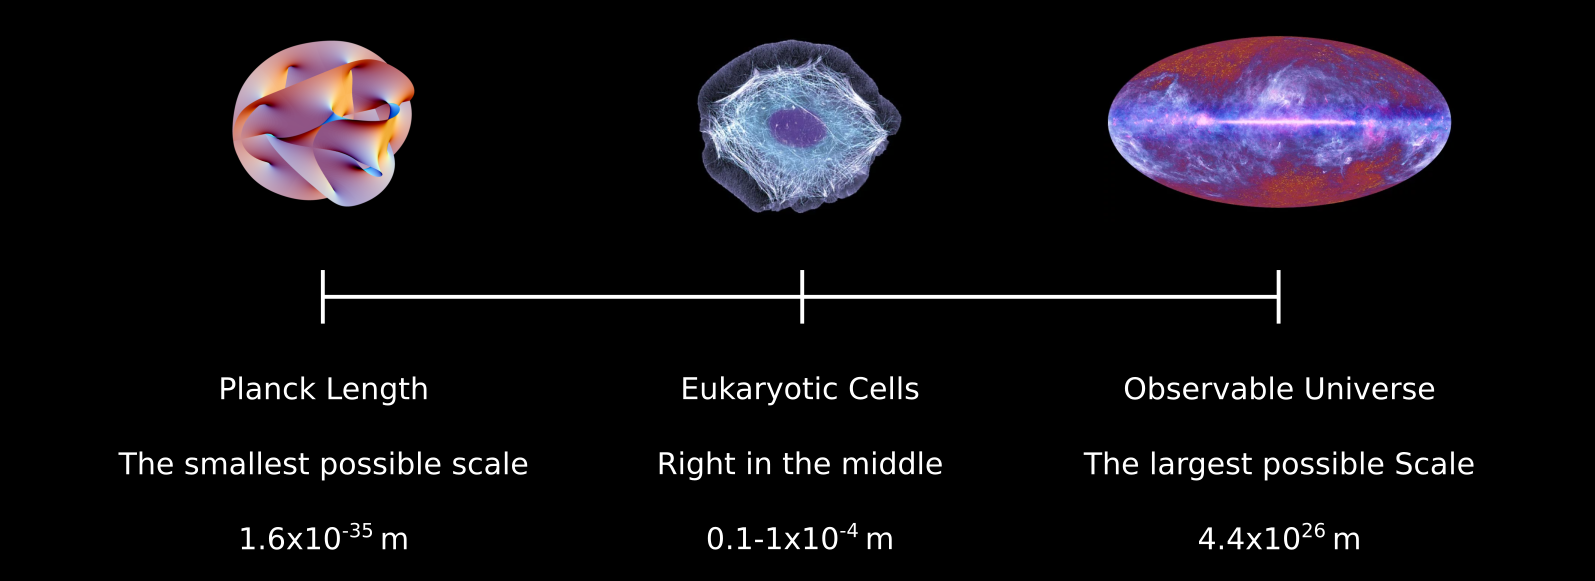
\includegraphics[width=1.0\textwidth]{figures/scales.png}
	\end{center}
	\captionsetup{singlelinecheck = false, justification=raggedright}
	\caption[The Position That Biology Occupies Compared to the Rest of Physics] {\textbf{The Position That Biology Occupies Compared to the Rest of Physics}}{It just so happens that if you plot the size of everything  in the universe on a log scale, eukaryotic cells fall right in the middle. A physicist can talk about both ends of this scale, we should learn something about the middle too.}
	\label{length_scales}
\end{figure}

Biological systems are not homogeneous. If you look at your hand, you will notice hair, pores, dry skin, dead skin, perhaps even tendons and muscles twitching beneath a ghostly web of blood vessels. If you were to pluck a single cell from anywhere in this hierarchy and view it under a microscope, you would just be able to make out some of the organelles inside that cell. The size, shape and function of the organelles would vary depending on what kind of cell you happened to choose. Within and between each those organelles is a wet, salty dance of molecular machines called proteins. It is this kind of molecule which I have trained to study in detail with computational models. The length scale of this journey, from your arm to a single protein, spans 8 orders of magnitude.\footnote{ From the size of your hand to the size a single protein spans from $10^{-1}$m  to $10^{-9}$m respectively.} At each step along the way, if you searched the literature your would find an army of experts studying an array of phenomenon at each length scale. 

Note for example how the publications arising from this thesis have many authors. Each researcher specialises, not unlike their cells, in a specific discipline. It is only by working together that can we hope to understand the whole organism.

%\footnote{I just noticed that the words organ, organism and organisation all contain the Greek root ``organon" meaning ``tool". Someone should look into that. }

%\interfootnotelinepenalty=10000
If the reader is anything like myself they will find the amount of required knowledge to study biology a substantial barrier to entry. It is quite difficult at first to figure out which questions to ask or even which subfields to study to alleviate confusion. These challenges can be tackled by cultivating a broad coalition of connections---speak to physicians, clinicians, evolutionary biologists \cite{dawkins1989, dawkins2016}, philosophers, molecular biologists, biochemists, cell biologists\cite{pollard2016}, geneticists, bioinformaticians, theoretical chemists, computer scientists, neuroscientists, physicists, mathematicians-everybody. It will take time but remain patient and you will find that a physics motivated approach can indeed explain and eventually even predict outcomes in biological experiments. A broad world view awaits you and it's really quite fun. 

%If the reader is anything like myself they will find the amount of required knowledge to study biology a substantial barrier to entry. It is quite difficult at first to figure out what questions to ask or even figure out which subfields to study to alleviate this confusion. These challenges can be tackled by cultivating a broad coalition of connections; speak to medical doctors, clinicians, evolutionary biologists \cite{dawkins1989, dawkins2016}, philosophers, molecular biologists, biochemists\footnote{These last two are in fact different subfields but like many in this list it'll take you some time to understand the subtle differences which define each one.\enlargethispage{-\baselineskip}}, cell biologists, geneticists, bioinformaticians, theoretical chemists, computer scientists, neuroscientists, physicists, mathematicians, everyone. It will take time but remain patient and you will find that a physics motivated approach can indeed explain and eventually predict outcomes in biological experiments. A broad world view awaits you and it's really quite fun. 

If this is indeed read by a future trainee, I hope the physics focussed philosophy in the introduction of chapter \ref{chap:introduction} and the literature review of simulation techniques in chapter \ref{chap:methods} can serve as a road map---but a physicist studying biology will also be served well by nurturing a strong base in electrodynamics and statistical mechanics \cite{griffiths2017, reif2009, zuckerman2010}. One particularly thorny issue for such a reader is that the field is now progressing so quickly that I'm sure much of this thesis will be out of date by the time it is read by anybody I would hope to train. But really, that's just one of the things that makes biophysics so exciting. Shoot me an email if you want help \href{mailto:miro.astore@gmailcom}{miro.astore@gmail.com}. Hopefully I'm still in the biophysics game.

The task ahead is immense. We're still not exactly sure how many unique proteins are expressed by the human genome, but it's upward of 20 thousand \cite{salzberg2018}. By contrast, this thesis represents an all consuming effort by a single PhD student---running decades worth of simulations to make incremental progress in the study of just one of these genes. There is so much to do. Good luck, I suggest you pack a towel \cite{adams1979}. 
